% Chapter Template

\chapter{Gene circuit design and parametrisation}
There is interest to build turing patterns in gene circuits. Synthetic biology can be used for that. Models are needed of synthetic biology circuits to understand dynamic behaviour, how to tune parameters for turing. These models can be parametrised to get them closer to synbio.

In this chapter we (1) present the model, (2) we look at the parameter space and what fraction of it leads to turing / how to tune the circuit to get more turing (3) parametrise the model with experimental dose response curves after the informed decision using machine learning.
\section{Building model describing synthetic gene circuit}
In this section, I present the model that describes the synthetic gene circuit engineered in~\cite{Tica2020}.
The circuit can be seen in Fig.~\ref{fig:synthetic circuit_chapter2}, which was already presented in the Introduction chapter but is repeated here to facilitate access to the reader.
Additionally, extra detail is added on the tuning molecules and receptor cassetes needed for full functioning of the circuit.

\begin{figure}[H]
    \centering
    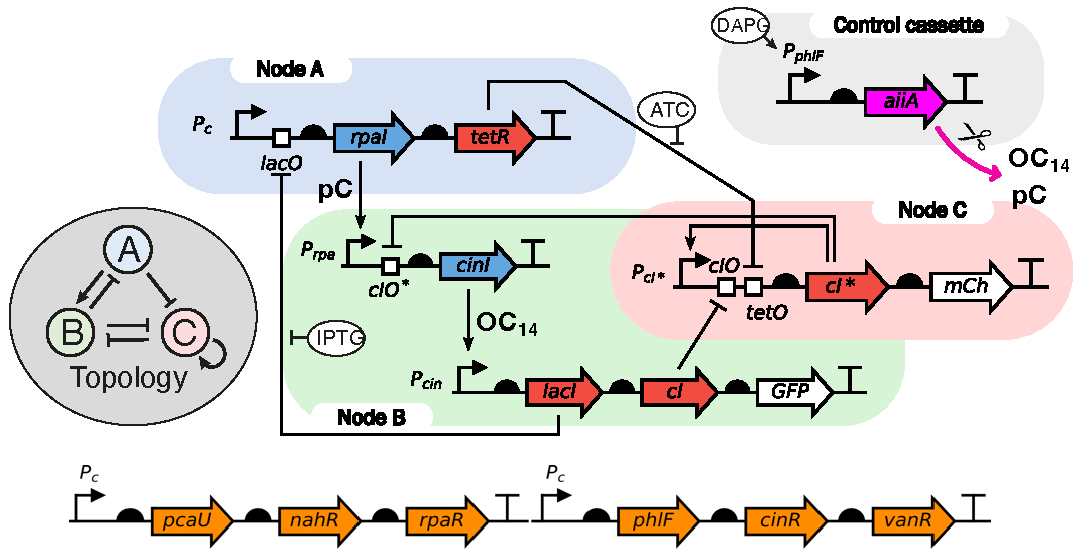
\includegraphics[width=1\textwidth]{chapters/Chapter 2/synthetic circuit2}
    \caption[\textbf{Synthetic biology implementation of 3954) topology.}]{\textbf{Synthetic biology implementation of 3954 topology.} \TODO{Give more detail of this diagram}} %TODO give detail
    \label{fig:synthetic circuit_chapter2}
\end{figure}


A PDE system is used to describe the reaction and diffusion terms, which describe change in concentrations of molecules in time and space.
This model includes constant background production, activator/repressor-regulated production using Hill terms, and the effect of tuning molecules aTc and IPTG on the circuit and diffusion.
The dynamics of the protein (X) and diffuser (U) species of the gene circuit are modeled as

\begin{subequations}\label{eq:Generalised protein and diffuser pde}
\begin{equation}
    \pdv{[X]}{t}= b_{X}+V_{X}\cdot\frac{1}{1+\left(\frac{K{A}}{[A]}\right)^{n_{A}}}\cdot\frac{1}{1+\left(\frac{[I]}{K_{I}}\right)^{n_{I}}}-\mu_{X}\cdot[X]
    \label{eq:Generalised protein}
\end{equation}

\begin{equation}
    \pdv{[U]}{t} = k_{1}\cdot[A] - \mu_{U}\cdot[U] + D_{U}(\partial_{xx} + \partial_{yy})[U]
    \label{eq:generalised diffuser}
\end{equation}
\end{subequations}

This results in a PDE model with eight equations that correspond to the two diffusers (pC and OC14) and six protein species of the circuit: RpaI, CinI, TetR, LacI, cI* and cI. This PDE model is reduced to a 6-equation system by assuming quasi-steady state for the diffusers, with production and degradation kinetics much faster than those of proteins. Finally, the model is non-dimensionalised to enable its parametrisation using liquid culture dose response data.
In the subsections below, the different terms of Eq.~\ref{eq:Generalised protein and diffuser pde} are discussed. Furthermore, the process of model reduction, non-dimensionalisation and fitting is also described.


\subsection{Protein equations and gene regulation}
The rate of protein production can be defined as
\begin{equation}
    V = V_{max} \cdot \theta
    \label{eq: vmax}
\end{equation}
where $\theta$ represents the fractional activation of the system. Full activation of protein production is denoted as $\theta=1$ while full inhibition is represented by $\theta=0$.
$V_{\max}$ is the maximal rate of expression.
$\theta$ can be represented by a Hill function to describe cooperative binding, derived using the law of mass action with all-or-none binding to multiple binding sites ~\parencite{Weiss1997}.
We further apply the quasi-steady state assumptions for activator and inhibitor binding to the promoter, as well as for the mRNA dynamics, as these timescales are much faster than protein production ~\parencite{Andersen1998, Bremer2008}.
This leads to the following expression of $\theta$ for non-competitive activation (A) and inhibition (I)
\begin{equation}
    \theta= \frac{1}{1+\left(\frac{K_{A}}{[A]}\right)^{n_{A}}} \cdot \frac{1}{1+\left(\frac{[I]}{K_{I}}\right)^{n_{I}}}
    \label{eq:theta}
\end{equation}
This Hill function is used in the Eq.~\ref{eq:Generalised protein} and describes promoter activity as a function of the two inputs [A] and [I], where $K_{A}$ and $K_{I}$ are half-activation/inhibition concentrations, $n_{A}$ and $n_{I}$ are the Hill coefficients.
Additionally, most promoters are leaky, which we account for by introducing a small rate of background production $b_{X}$. $b_{X}$ corresponds to the first term in Eq.~\ref{eq:Generalised protein}

\begin{figure}[H] % h! is a placement specifier; it tries to place the image here.
    \centering
    \begin{adjustbox}{center}
        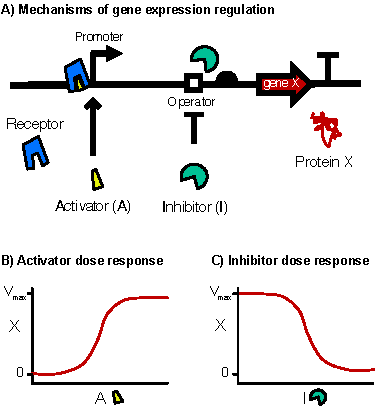
\includegraphics[width=0.7\textwidth]{chapters/Chapter 2/activation_inhibition} % The name of your image file; assumes it's in the same directory as your .tex file
    \end{adjustbox}
    \caption{\textbf{Activation and Inhibition of gene expression.} Activator generally works by binding a receptor which then binds the promoter to activate gene expression. Inhibitor generally works by binding the operator and inhibiting gene expression. In the case of this model, activators are diffusers (pC, $OC_{14}$) with their respective receptors (RpaR, CinR) and inhibitors are proteins (RpaI, CinI, TetR, LacI, cI, cI*) }. %TODO fact check}
    \label{fig:activation_inhibition} % A label for referencing this figure later in the document
\end{figure}

A visual representation of the mechanisms of activation and inhibition modelled in Eq.~\ref{eq:theta} can be observed in Fig.~\ref{fig:activation_inhibition} .


\subsection{Tuning gene expression: aTc regulation of TetR and IPTG regulation of LacI }



%The circuit was designed so it can be tuned in a variety of ways.
Experimentally, the circuit was designed to be tuned n a variety of ways using aTc, IPTG and DAPG.
This tuning was used to achieve parameter combinations that are more favourable for patterning.
The following section introduces aTc and IPTG tuning into the model.

\begin{figure}[H] % h! is a placement specifier; it tries to place the image here.
    \centering
    \begin{adjustbox}{center}
        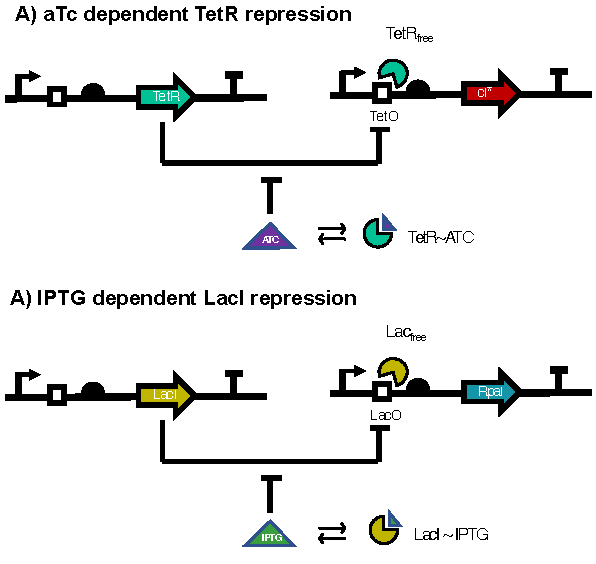
\includegraphics[width=0.7\textwidth]{chapters/Chapter 2/inducers} % The name of your image file; assumes it's in the same directory as your .tex file
    \end{adjustbox}
    \caption{Inducer dependent repressions using aTc and IPTG for circuit tuning}
    \label{fig:inducers} % A label for referencing this figure later in the document
\end{figure}

As shown in Fig.~\ref{fig:inducers}A, aTc binds to TetR and inactivates it.
Only free, unbound TetR can bind TetO and inactivate the expression of cI*.
The binding of aTc to TetR is modelled by a reversible equilibrium.
The affinity of binding is given by the $k_{on}$ and $k_{off}$ rate constants.



\begin{equation}
    aTc + TetR_{free} \xrightleftharpoons[k_{off}]{k_{on}} TetR \mhyphen aTc
\end{equation}

This equilibrium happens at much faster rates than the protein production and degradation reactions of the model.
For this reason, quasi-steady state is assumed

\begin{equation}
    \pdv{TetR \mhyphen aTc}{t} = k_{on}[TetR_{free}][aTc]^n - k_{off}[TetR \mhyphen aTc] \approx 0
\end{equation}


By rearranging terms and using $K_{d} = k_{off}/k_{on}$, a simplified expression for $[TetR_{free}]$ is obtained, which is then used in the model

\begin{equation}
[TetR_{free}] = K_{D}\cdot \frac{[TetR \mhyphen naTc]}{[aTc]^n}
\end{equation}

However, because $[TetR-naTc]$ is unknown, the $[TetR_{total}]$ and $[TetR_{free}]$ are used instead

\begin{equation}
[TetR \mhyphen naTc] = [TetR_{total}] - [TetR_{free}]
\end{equation}

to obtain the following expression

\begin{subequations}
    \begin{equation}
    [TetR_{free}] = K_{D} \cdot \frac{[TetR_{total}] - [TetR_{free}]}{[aTc]^n} \Longrightarrow
    \end{equation}
    \begin{equation}
    [TetR_{free}] (1+\frac{K_{D}}{[aTc]^n}) = \frac{K_{D}\cdot [TetR_{total}]}{[aTc]^n}\Longrightarrow
    \end{equation}
    \begin{equation}
    [TetR_{free}] = \frac{K_{D}\cdot[TetR_{total}]}{[aTc]^n+K_{D}} = \frac{[TetR_{total}]}{1+\frac{[aTc]^n}{K_{D}}}
    \end{equation}
\end{subequations}

which says that the concentration of unbound TetR is given by ~$[aTc]$, ~$[TetR_{total}]$ and the equilibrium constant ~$K_{D}$.

For non-cooperative systems where ~$n=1$, ~$K_{D}=[L_{half}]$.
However, for cooperative systems where ~$n>1$, ~$[L_{half}] = \sqrt[n]{K_{D}}$.
We define a new variable ~$K_{A} = \sqrt[n]{K_{D}} \leftrightarrow K_{D} = K^n_{A}$ that we use to replace ~$K_{D}$ in the following expression, where ~$K^n_{A} = K_{TetR \mhyphen naTc}{[aTc]^n}$.
This was also done for other ~$K_{D}$ parameters of the model.
\begin{equation}
[TetR_{free}] =  \frac{[TetR_{total}]}{1+(\frac{[aTc]}{K_{TetR \mhyphen aTc}})^{n_{aTc}}}
\end{equation}
Parameter ~$K_{TetR \mhyphen aTc}$ is the binding affinity of aTc to TetR, whereas $n_{aTc}$ is the cooperativity of TetR and aTc binding.
This expression for unbound TetR ($[TetR_{free}]$ ), can then be introduced into the production rate of cI*.
cI* has an operator sequence downstream of the promoter, TetO.
This TetO is bound by TetR to inhibit expression of the mRNA. We will model the production of cI* dependent of TetR binding, using an inverse-Hill term that describes repression by this binding as described by Eq.~\ref{eq: vmax} and Eq.~\ref{eq:theta}.

\begin{equation}
    \pdv{[cI*]}{t} = V_{max}\cdot \left(1+\left(\frac{[TetR_{free}]}{K_{TetR \mhyphen TetO}}\right)^{n_{TetO}}\right)^{-1} = V_{max} \cdot \left(1+\left(\frac{TetR_{total}}{K_{TetR \mhyphen TetO}\cdot(1+(\frac{aTc}{K_{TetR \mhyphen aTc}})^{n_{aTc}})}\right)^{n_{TetO}}\right)^{-1}
\end{equation}

We can simplify the denominator so

\begin{equation}
    \pdv{[cI*]}{t} = V_{max}\cdot \left(1+\left(\frac{[TetR_{free}]}{K_{TetR \mhyphen TetO \mhyphen aTc }}\right)^{n_{TetO}}\right)^{-1}
\end{equation}

where,

\begin{equation}
    K_{TetR \mhyphen TetO \mhyphen aTc }=K_{TetR \mhyphen TetO}\cdot(1+(\frac{aTc}{K_{TetR \mhyphen aTc}})^{n_{aTc}})
\end{equation}

%\TODO{Explain different params here above}

The parameter $K_{TetR \mhyphen TetO \mhyphen aTc }$ is the binding affinity of TetR to TetO, $K_{TetR \mhyphen aTc}$ is the affinity of aTc to TetR, $n_{aTc}$ is the Hill coefficient of aTc and TetR, and $n_{TetO}$ is the Hill coefficient of TetR to TetO.
Therefore, the higher the aTc, the higher the production of cI*.

The same logic can be applied for the IPTG regulating LacI inhibition (See Fig.~\ref{fig:inducers}B), where unbound LacI can be or $[LacI_{free}]$ can be expressed as
\begin{equation}
[LacI{free}] =  \frac{[LacI_{total}]}{1+(\frac{[IPTG]}{K_{LacI \mhyphen IPTG}})^{n_{IPTG}}}
\end{equation}

LacI free will be then able to bind to LacO and inhibit RpaI and tetR production in the following manner

\begin{equation}
    \pdv{[RpaI]}{t} = V_{max}\cdot \left(1+\left(\frac{[LacI_{free}]}{K_{LacI \mhyphen LacO}}\right)^{n_{LacO}}\right)^{-1} = V_{max} \cdot \left(1+\left(\frac{LacI_{total}}{K_{LacI \mhyphen LacO}\cdot(1+(\frac{IPTG}{K_{LacI \mhyphen IPTG}})^{n_{IPTG}})}\right)^{n_{LacO}}\right)^{-1}
\end{equation}


We can again simplify the denominator so

\begin{equation}
    \pdv{[RpaI]}{t} = V_{max}\cdot \left(1+\left(\frac{[LacI_{free}]}{K_{LacI \mhyphen LacO \mhyphen IPTG }}\right)^{n_{LacO}}\right)^{-1}
\end{equation}

where,

\begin{equation}
    K_{LacI \mhyphen LacO \mhyphen IPTG} = K_{LacI \mhyphen LacO}\cdot(1+(\frac{IPTG}{K_{LacI \mhyphen IPTG}})^{n_{LacO}})
\end{equation}

The parameter $K_{LacI \mhyphen LacO \mhyphen IPTG}$ is the binding affinity of TetR to TetO, $K_{LacI \mhyphen IPTG}$ is the affinity of IPTG to LacI, $n_{IPTG}$ is the Hill coefficient of IPTG and LacI, and $n_{LacO}$ is the Hill coefficient of LacI to LacO. Therefore, the higher the IPTG, the higher the production of RpaI.




\subsection{Degradation}
All the species of the circuit, including proteins and diffusers, were modelled to undergo linear (first order) degradation
\begin{equation}
    -\mu_{P_{1}}[X]
    \label{linear degradation}
\end{equation}

as seen in Eq.~\ref{eq:Generalised protein and diffuser pde}.
The degradation rate parameters for the protein species and diffusers are readily available in the literature~\parencite{Andersen1998,Kaufmann2005} and can be found in Table~\ref{table:degradation table}.
They are scale-free parameters that only depend on time, which makes them more translatable between different experimental contexts and units of measurement. %TODO issue with references here


\begin{table}[H]
    \centering
    \begin{tabular}{|c|c|c|}
        \hline
        Degradation tag & Species 2 & Rate $[h^{-1}]$ \\
        \hline
        LVA 1 & CinI, LacI, cI, cI*, TetR 1 & 1.14 \\
        ASV & RpaI, GFP, mCherry 3 & 0.30 \\
        Diffusers & pC, $OC_{14}$ & 0.0225 \\
        \hline
    \end{tabular}
    \caption{\textbf{Degradation Parameters.} Degradation coefficients of protein species with degradation tags LVA and ASV, and basal degradation of diffusers.}
    \label{table:degradation table}
\end{table}

The proteins of the circuit were added short peptide sequences at their 3’ ends, known as degradation tags, that promote their breakdown by the cell’s proteolytic enzymes.
The diffusors degradation could be further induced by adding exogenous DAPG to the system which induces degradation by AiiA lactonase.






\subsection{Diffuser equations}
Diffusers are synthesised by enzymes, and then bound to receptors to activate gene expression by binding to the promoter (See Fig.~\ref{fig:activation_inhibition}). %check if its true they bind to the promoter.
The circuit receptors are expressed constructively from a low-copy pCC1 plasmid, and are therefore modelled with a constant concentration.
Quasi-steady state was assumed for the very fast equilibrium that forms between the receptor and the diffusers.
The receptor-inducer and receptor-promoter binding equilibria were modelled with mass action kinetics.
%TODO comment on concentrations of receptors

The enzymatic production of the diffusers was modelled with a simple linear production term dependent on synthesis enzyme concentration ([A], [B]), and a rate constant ($K_{1}$ and $K_{2}$).
It is assumed that the precursor substrate concentration is in excess and does not influence the reaction rate.


The diffusers are also modelled to undergo linear degradation, parameterised by $\mu_{U}$ and $\mu_{V}$ as seen in Eq.~\ref{linear degradation}. This degradation is a combination of a spontaneous hydrolysis in water, enzymatic AiiA-dependent degradation, and other cellular metabolic processes %~\parencite{Kaufmann2005},~\parencite{Wang2004},  \parencite{Momb2008}. %TODO add ref

Finally, the diffuser movement through space is modelled with simple diffusion terms and parameterised with diffusion coefficients $D_{U}$ and $D_{V}$.

\begin{subequations}\label{diffuser}
\begin{equation}
    \pdv{[U]}{t} = k_{1}\cdot[A] - \mu_{U}\cdot[U] +  D_{U}(\partial_{xx} + \partial_{yy})[U]
\end{equation}
\begin{equation}
    \pdv{[V]}{t} = k_{2}\cdot[B] - \mu_{V}\cdot[V] + D_{V}(\partial_{xx} + \partial_{yy})[V]
\end{equation}
\end{subequations}

The time dynamics of diffuser synthesis is much faster than that of protein production.
Therefore, the rate of change of diffuser is expected to be much higher than that of proteins.
These rapid fluctuations of diffuser can be approximated to equilibrium by using the quasi-steady state approximation, meaning the rate is set to zero.
This leads to an expression of diffuser concentration that is linearly correlated with their synthesis enzyme and rate constant, and inversely correlated with their degradation rate.

\begin{subequations}\label{diffuser quasi-steady state}

\begin{equation}
    \pdv{[U]}{t} = k_{1}\cdot[A] - \mu_{U}\cdot[U] = 0
    \longrightarrow U = \frac{k_{1}}{ \mu_{U}}[A]
\end{equation}

\begin{equation}
    \pdv{[V]}{t} = k_{2}\cdot[B] - \mu_{V}\cdot[V] = 0
    \longrightarrow V = \frac{k_{2}}{ \mu_{V}}[B]
\end{equation}
\end{subequations}

In this process, the diffusion of U and V is artificially assigned to A and B, since

\begin{subequations}\label{[diffuser_artificial]}

\begin{equation}
    U = \frac{k_{1}}{ \mu_{U}}[A] \longrightarrow D_{U} (\partial_{xx} + \partial_{yy})[U] = D_{U}\frac{k_{1}}{ \mu_{U}}  (\partial_{xx} + \partial_{yy}) [A]\label{eq:equation2}
\end{equation}

\begin{equation}
    V = \frac{k_{2}}{ \mu_{V}}[B] \longrightarrow D_{V} (\partial_{xx} + \partial_{yy})[V] =  D_{V}\frac{k_{2}}{ \mu_{V}}  (\partial_{xx} + \partial_{yy}) [B]\label{eq:equation}
\end{equation}

\end{subequations}

These quasi-steady state expressions are used to model the diffusers implicitly within the gene equations.
Therefore, instead of using eight equations for the six genes and two diffusers; we have six equations for the six genes with the two diffusers modelled implicitly.
U and V will be modelled within A and B in the Hill activation and diffusion terms

\begin{equation}
    \pdv{[A]}{t} = b_{A}+V_{A}\cdot \frac{1}{\left(1+\left(\frac{[I]}{K_{I}}\right)^{n_{I}}\right)}-\mu_{A}\cdot[A] + \frac{ k_{1}D_{U}}{ \mu_{U}}\cdot (\partial_{xx} + \partial_{yy})[A]
\end{equation}

\begin{equation}
    \pdv{[B]}{t} = b_{B}+V_{B}\cdot\frac{1}{1+\left(\frac{\mu_{u}K{ub}}{k_{1}[A]}\right)^{n_{ab}}}\cdot\frac{1}{1+\left(\frac{[I]}{K_{I}}\right)^{n_{I}}}-\mu_{B}\cdot[B] + \frac{ k_{2}D_{V}}{ \mu_{V}}\cdot (\partial_{xx} + \partial_{yy})[B]
\end{equation}

Although these genes are not explicitly modelled, a linear relationship between downstream genes in the same operon
\subsection{Six-equation model}
We combined all the terms described above including the basal production, activator or inhibitor regulated production, tuning molecules, linear degradation and implicit diffusers.
All these terms are applied to the circuit shown in Fig %TODO ref figure.
This results in a 6 equation model with information on the 6 proteins in space and time

\begin{subequations}\label{[6 equation proteins]}

\begin{equation}
    \pdv{[A]}{t} = b_{A}+V_{A}\cdot \frac{1}{\left(1+\left(\frac{[D]}{K_{da}}\right)^{n_{da}}\right)}-\mu_{A}\cdot[A] + \frac{ k_{1}D_{U}}{ \mu_{U}}\cdot (\partial_{xx} + \partial_{yy})[A]
\end{equation}

\begin{equation}
    \pdv{[B]}{t} = b_{B}+V_{B}\cdot\frac{1}{1+\left(\frac{\mu_{u}K{ub}}{k_{1}[A]}\right)^{n_{ab}}}\cdot\frac{1}{1+\left(\frac{[E]}{K_{eb}}\right)^{n_{eb}}}-\mu_{B}\cdot[B] + \frac{ k_{2}D_{V}}{ \mu_{V}}\cdot (\partial_{xx} + \partial_{yy})[B]
\end{equation}

\begin{equation}
    \pdv{[C]}{t} = b_{C}+V_{C}\cdot \frac{1}{\left(1+\left(\frac{[D]}{K_{da}}\right)^{n_{da}}\right)}-\mu_{C}\cdot[C]
\end{equation}

\begin{equation}
    \pdv{[D]}{t} = b_{D}+V_{D}\cdot\frac{1}{1+\left(\frac{\mu_{V}K{vd}}{k_{2}[B]}\right)^{n_{bd}}}-\mu_{D}\cdot[D]
\end{equation}

\begin{equation}
    \pdv{[E]}{t} = b_{E}+V_{E}\cdot \frac{1}{\left(1+\left(\frac{[C]}{K_{ce}}\right)^{n_{ce}}\right)}\cdot\frac{1}{1+\left(\frac{[F]}{K_{fe}}\right)^{n_{fe}}}\cdot\frac{1}{1+\left(\frac{K{ee}}{[E]}\right)^{n_{ee}}}-\mu_{E}\cdot[E]
\end{equation}

\begin{equation}
    \pdv{[F]}{t} = b_{F}+V_{F}\cdot\frac{1}{1+\left(\frac{\mu_{V}K_{bd}}{k_{2}[B]}\right)^{n_{bd}}}-\mu_{F}\cdot[F]
\end{equation}

\end{subequations}

where $K_{da}$ and $K_{ce}$ are expressed in terms of the tuning molecules such as

\begin{subequations}
    \begin{equation}
        K_{da} = K_{lacI-lacO} \left( 1 + \frac{[IPTG]}{K_{lacI-IPTG}}\right)^{n_{IPTG}}
    \end{equation}

    \begin{equation}
        K_{ce} = K_{tetR-tetO} \left( 1 + \frac{[aTc]}{K_{tetR-aTc}}\right)^{n_{aTc}}
    \end{equation}
\end{subequations}

The six dependent variables can be found in Table~\ref{tab:Model variables}.
They can be thought of as protein concentrations, although they are also directly linked to the gene expressed to produce that protein.
The units are nM.
\begin{table}[H]
    \centering
    \caption{Model variables}
    \label{tab:Model variables}
    \renewcommand{\arraystretch}{1.3} % Adjust vertical padding
    \begin{tabular}{|c|c|c|}
        \hline
        \textbf{Variable} & \textbf{Biological molecule} & \textbf{Node in original 3-node circuit}\\
        \hline
        [A] & RpaI & A\\
        \hline
        [B] & CinI & B \\
        \hline
        [C] & TetR & A\\
        \hline
        [D] & LacI & B \\
        \hline
        [E] & cI* & C \\
        \hline
        [F] & cI & B \\
        \hline
    \end{tabular}
\end{table}
Description of the parameters used in the model can be found in Table~\ref{tab:Model variables}.

\begin{table}[H]
    \centering
    \caption{Model parameters}
    \label{tab:variables}
    \renewcommand{\arraystretch}{1.3} % Adjust vertical padding
    \begin{tabular}{|c|c|c|}
        \hline
        \textbf{Parameter} & \textbf{Description} & Units\\
        \hline
        $t$ & Time & t\\
        \hline
        $x$ & Space & mm\\
        \hline
        $b_{X}$ & Background production rate of X & nM/h\\
        \hline
        $V_{X}$ & Induced max production rate of X & nM/h \\
        \hline
        $K_{XY}$ & Dissociation constant of X binding to Y regulator DNA & nM \\
        \hline
        $n_{XY}$ & Cooperativity constant of X binding to Y regulator DNA & 1\\
        \hline
        $\mu_{X}$ & Degradation rate of X & 1/h\\
        \hline
        $D_{X}$ & Diffusion rate of diffuser X & $mm^2/h$\\
        \hline

    \end{tabular}
\end{table}

For $K_{XY}$ and $n_{XY}$, activators X will bind to a receptor molecule that binds the promoter sequence upstream of gene Y; while inhibitors X will bind to the operator sequence upstream of gene Y.



\subsection{Dimensionless Six-equation model}

A dimensionless model (or non-dimensional model) is derived to better understand the nature of the parameters, and to simplify the fitting process, as explained below.
The non-dimensionalisation involves the following transformations of dependent and independent variables of concentration (X), time (t) and space (x and y).


\begin{equation}\label{variable transformations}
    X = \frac{b_{x}}{\mu_{x}}X^*, t = \frac{t^*}{\mu_{a}},
    x = \sqrt{\frac{k_{1}D_{u}}{\mu_{a}\mu_{u}}}x^*, y = \sqrt{\frac{k_{1}D_{u}}{\mu_{a}\mu_{u}}}y^*
\end{equation}

And the following transformations of the system parameters V, µ, K and D:

\begin{equation}\label{parameter transformations}
    V_{x}^*=\frac{V_{x}}{b_{x}},  \mu_{x}^* = \frac{\mu_{x}}{\mu_{a}}, K^*_{yx} = \frac{\mu_{x}}{b_{x}}K ,D_{r} = \frac{k_{2}D_{v}\mu_{u}}{k_{1}D_{u}\mu_{v}}
\end{equation}

It is important to note that time and degradation of all species is now relative to the degradation rates of A (RpaI) which is an estimated parameter from the literature (See Table~\ref{table:degradation table}).
If this parameter changes over the course of the experiment, the effects should be absorbed by the dimensionless model.

If those transformations are applied to the original six-equation model shown in Eqs.~\ref{[6 equation proteins]} the following dimensionless model is obtained

\begin{subequations}\label{six_eq_dimensionless}

    \begin{equation}
        \pdv{[A^*]}{t^*} = 1 + V_{a}^* \left(\frac{1}{1+\left(\frac{[D^*]}{K_{da}^*}\right)^{n_{da}}}\right) - [A^*] + (\partial_{xx} + \partial_{yy})[A^*]
    \end{equation}

    \begin{equation}
        \pdv{[B^*]}{t} =\mu_{b}^* \left(1+V_{B}^*\left(\frac{1}{1+\left(\frac{\mu_{u}K{ub}^*}{k_{1}[A^*]}\right)^{n_{ab}}}\right)\cdot\left(\frac{1}{1+\left(\frac{[E^*]}{K_{eb}^*}\right)^{n_{eb}}}\right) -[B^*] \right)+ D_{r}(\partial_{xx} + \partial_{yy})[B^*]
    \end{equation}

    \begin{equation}
        \pdv{[C^*]}{t^*} = \mu_{c}^*\left(1 + V_{c}^* \left(\frac{1}{1+\left(\frac{[D^*]}{K_{da}^*}\right)^{n_{da}}}\right) - [C^*]\right)
    \end{equation}

    \begin{equation}
        \pdv{[D^*]}{t^*} = \mu_{d}^*\left(1 + V_{d}^* \left(\frac{1}{1+\left(\frac{\mu_{v}K_{vd}^*}{k_{2}[B^*]}\right)^{n_{vd}}}\right) - [D^*]\right)
    \end{equation}
    \begin{equation}
        \pdv{[E^*]}{t^*} = \mu_{e}^*\left(1 + V_{e}^* \left(\frac{1}{1+\left(\frac{[C^*]}{K_{ce}^*}\right)^{n_{ce}}}\right)\left(\frac{1}{1+\left(\frac{[F^*]}{K_{fe}^*}\right)^{n_{fe}}}\right)\left(\frac{1}{1+\left(\frac{K_{ee}^*}{[E^*]}\right)^{n_{ee}}}\right)  - [E^*]\right)
    \end{equation}
    \begin{equation}
        \pdv{[F^*]}{t^*} = \mu_{f}^*\left(1 + V_{f}^* \left(\frac{1}{1+\left(\frac{\mu_{v}K_{vd}^*}{k_{2}[B^*]}\right)^{n_{vd}}}\right) - [F^*]\right)
    \end{equation}

\end{subequations}

A summary of the model parameters including notation, original units and dimensionless units can be found in Table~\ref{tab:Dimensionless_params}.


\begin{table}[H]
    \centering
    \caption{Dimensionless model parameters}
    \label{tab:Dimensionless_params}
    \renewcommand{\arraystretch}{2.3} % Adjust vertical padding
    \begin{tabular}{|c|c|c|c|}
        \hline
        \textbf{Parameter} & \textbf{Description} & \textbf{Original Units} & \textbf{Dimensionless Units} \\
        \hline
        $X^*$ & Molecular species & $nM$ & $\frac{\mu_{x}}{b_{x}}X \quad \rightarrow \quad  \frac{nM/h}{nM/h}  = 1$
        \\
        \hline

        $OC_{14}$ & NodeB inducer & $nM$ & $\frac{k_{2} b_{B}}{\mu_{v} \mu_{b}} B^* \quad \rightarrow \quad  1$
        \\
        \hline
        $b_{x}^*$ & Background production rate & $nM/h$ & no $b_{x} $\\
        \hline
        $ V_{x}^*$  & Induced max production rate & $nM/h$ & $ \frac{V_{x}}{b_{x}} \quad \rightarrow \quad  \frac{nM/h}{nM/h} = 1 $\\
        \hline
        $K_{yx}^*$ & Dissociation constant & $nM$ & $ \frac{\mu_{x}}{b_{x}} K_{yx} \quad \rightarrow \quad \frac{nM/h}{nM/h} = 1 $\\
        \hline
        $ n_{yx}$  & Cooperativity constant & 1 & 1\\
        \hline
        $ \mu_{x}^* $ & Degradation rate & $1/h$ & $\frac{\mu_{x}}{\mu_{a}} \quad \rightarrow \quad  \frac{1/h}{1/h}=1 $\\
        \hline
        $D_{x}$ & Diffusion rate & $mm/h$ & $ \frac{k_{2} D_{v} \mu_{u}}{k_{1} D_{u} \mu_{v}} \quad \rightarrow \quad  1$  \\
        \hline
        $ t $ & Time & $h$ & $\mu_{a} \cdot t \quad \rightarrow \quad  h \cdot  h^{-1} =1$\\
        \hline
        $ x$  & Space & $mm$ & $\sqrt{\frac{k_{1} D_{1}}{\mu_{a}\mu_{v}} }/x \rightarrow  \sqrt{\frac{h^{-1} mm^{2} h^{-1}}{h^{-1}h^{-1}}}/mm  = 1$ \\
        \hline
    \end{tabular}
\end{table}

\subsection{Fluorescence reporters}
In addition to the six genes involved in circuit regulation, there are two fluorescent reporter genes: GFP and mCherry.
GFP is in the same operon as lacI and cI, meaning a single mRNA is transcribed with the three genes.
The difference is that each have their own Ribosome Binding Site (RBS), so they are translated into proteins independently.
Therefore, we can assume GFP is linearly correlated with lacI and cI.
The same thing can be inferred for mCherry and cI*.
Instead of modelling GFP and mCherry as two extra equations, lacI and cI* concentrations will be used instead when studying how the fluorescent distributions look like spatially

\begin{subequations}
    \begin{equation}
        [GFP] = \alpha_{GFP}*[LacI]
    \end{equation}
    \begin{equation}
        [mCherry] = \alpha_{mCherry}*[cI^*]
    \end{equation}
\end{subequations}

where $\alpha$ is the fractional translation between the two proteins in the same operon.


Both the dimensional and the non-dimensional 6 equation models (Eqs.~\ref{[6 equation proteins]} and Eqs.~\ref{six_eq_dimensionless}) are close representation of the synthetic gene circuit engineered by~\cite{Tica2020} shown in Fig.~\ref{fig:synthetic circuit_chapter2}.
The non-dimensional model (Eqs.~\ref{six_eq_dimensionless}) will be used to explore the potential of this gene circuit for pattern formation by studying GFP and mCherry distributions in an \textit{in-silico} tissue.



\section{Explore parameter space and optimise robustness}
Prior to performing any experiments on the gene circuit, I explored the parameter space of our system to understand which possible spatio-temporal dynamics could be generated by this circuit.
In particular, I investigated whether this 6 node synthetic biology implementation of the original 3 node-network from~\cite{Scholes2019} could produce Turing patterns.
Finally, I explored computationally how to tune the genetic circuit experimentally to maximise the probability of Turing pattern formation.

A biologically realistic parameter space was defined as follows:
A distribution for each parameter was generated, and the multi-dimensional parameter space was sampled using Latin Hypercube Sampling (See~\ref{sampling method}) \parencite{Iman2014, Bergstra2012}, which ,maximises the sampling efficiency with fewer samples.
Depending on the certainty of the parameter, different distributions were defined as seen in Table%TODO ref table
For certain parameters, For each parameter of the model, literature searches were carried out to define biologically realistic lower and upper bounds.



\begin{table}[H]
\caption{Model parameters}
\label{tab:param distributions}
\renewcommand{\arraystretch}{1.3} % Adjust vertical padding
\begin{tabular}{|c|p{45mm}|c|c|}
\hline
\textbf{Parameter} & \textbf{Description} & \textbf{Distribution} & \textbf{Value}\\
\hline

$V_{X}$ & Induced max production rate of X & Loguniform &  1-100 \\
\hline
$b_{X}$ & Background production rate of X & Loguniform & 0.1-1\\
\hline
$D_{U}, D_{V}$ & Diffusion rate of pC and $OC_{14}$ & Loguniform & 0.1-10\\
\hline
$K_{XY}$ & Dissociation constant of X binding to Y regulator DNA & Loguniform & 0.1-1000\\
\hline
$K_{ee}$ & Dissociation constant of cI* binding its own promoter ($P_{cI*}$) & Fixed & 0.01\\
\hline
$k_{1},k_{2}$ & pC and $OC_{14}$ production rate constants  & Fixed & 0.0183\\
\hline
$\mu_{u},\mu_{v}$ & pC and $OC_{14}$ degradation rates & Fixed & 0.0225\\
\hline
$\mu_{LVA}$ & Degradation rates of proteins with LVA tag (CinI, LacI, cI, cI*, TetR $\rightarrow \mu_{B}, \mu_{C}, mu_{D}, \mu_{E}, \mu_{F}$) & Gaussian & mean=1.143, std=mean*0.1\\
\hline
$\mu_{ASV}$ & Degradation rates of proteins with LVA tag (RpaI $\rightarrow \mu_{A}$) & Fixed & 0.3\\
\hline
$n_{ub}, n_{vd}$ & Cooperativity of pC and $OC_{14}$ with receptors binding binding to $P_{rpa}$ and $P_{cin}$ promoters respectively & Fixed & 1,2\\
\hline


\end{tabular}
\end{table}



%\section{Parametrise model to constrain}
%
%\section{Produce rings}
%\section{Modelling bacterial colonies}
%\subsection{openboundary circle shape growth noise}
%\section{Explore patterning potential}
%\subsection{general params}
%\subsection{parametrised params}
